\documentclass[conference]{IEEEtran}
\IEEEoverridecommandlockouts
% The preceding line is only needed to identify funding in the first footnote. If that is unneeded, please comment it out.
\usepackage{cite}
\usepackage{amsmath,amssymb,amsfonts}
\usepackage{algorithmic}
\usepackage{graphicx}
\usepackage{textcomp}
\usepackage{xcolor}
\usepackage[utf8]{inputenc}
\usepackage[vietnamese]{babel}
\addto\captionsvietnamese{%
  \renewcommand{\abstractname}{Abstract}
}
\usepackage{amsmath}
\usepackage{hyperref}
\usepackage{tabularx}
\usepackage{multirow}
\usepackage{multicol}
\usepackage{array} 
\usepackage[table,xcdraw]{xcolor} 
\usepackage{placeins}
\usepackage{tcolorbox}
\usepackage{verbatim}


\def\BibTeX{{\rm B\kern-.05em{\sc i\kern-.025em b}\kern-.08em
    T\kern-.1667em\lower.7ex\hbox{E}\kern-.125emX}}

\begin{document}

\title{A Study on Integrating Retrieval-Augmented Generation with Large Language Model for Consulting Support in Development and Mental Health of Children Under 6 Years Old}

\author{
Thanh Nguyen Van Quoc $^{1}$, Hao Nguyen Thi Bich $^{2}$, Nhut Nguyen Minh$^{3}$, Thuan Nguyen Dinh$^{4}$\\
\textit{Faculty of Information Systems} \\
\textit{University of Information Technology - Vietnam National University} \\
Ho Chi Minh City, Vietnam \\
\{21521447@gm.uit.edu.vn, 21522049@gm.uit.edu.vn, nhutnm.17@grad.uit.edu.vn, thuannd@uit.edu.vn\}
}


\maketitle


\begin{abstract}
    Currently, the need for psychological health as well as parents’ concerns about the rate of development of children is very high due to the growing number of cases of autism, Autism Spectrum Disorders (ASD), developmental delays have been discovered in recent years. However, most people are not well aware or well-gathered about this issue. Therefore, parents or relatives of the child have not yet given a correct objective assessment of these diseases. The use of the RAG framework, in conjunction with LangChain and using a Large Language Model (LLM) will help people learn and receive better results about mental health-related diseases and developmental milestones that children under 6 years old need to achieve
\end{abstract}
% \begin{IEEEkeywords}
% Currency exchange rates, Forecasting, Historical data, Predictive modeling, Financial decision-making, Linear Regression, ARIMA, RNN, GRU, LSTM, FFT, FEDformer, PatchTST, Boosting Model, TBATS
% \end{IEEEkeywords}
\section{Introduction}
\label{sec:introduction}
% Trong bối cảnh kinh doanh phát triển nhanh chóng ngày nay, phân tích dữ liệu đóng một vai trò then chốt trong quá trình ra quyết định giữa các ngành. 
With the continuous development of machine learning and deep learning, AI has been a powerful assistant in supporting people in most areas. The field of child mental health and development assessment is chosen by the team to learn, study the uses and challenges that an RAG, LangChain and LLM architecture can bring and encounter.

Our research objective is to apply the Retrieval-Augmented Generation framework (RAG) in combination with LangChain technology and outstanding LLM models for Vietnamese data. The aim is to assess the reliability and efficiency of these models when applied to the field of pediatric mental health and development. Selected LLM models include Viet-Mistral/Vistral-7B-Chat, SeaLLMs/SeaLLMs-v3-7B-Chat, vilm/vinallama-7b-chat and vietgpt/dama-2-7b-chat. Despite differences in model parameters, this study aims to assess the suitability of each model with the Vietnamese dataset, especially when using a relatively small amount of data to fine-tune. To evaluate model quality, we will use indicators such as METEOR, ROUGE and Cosine Similarity.

\section{Related Works}
\label{sec:Related Works}
Kailai Yang, Tianlin Zhang, Ziyan Kuang, Qianqian Xie, Jimin Huang, and Sophia Ananiadou \cite{b1} presented a paper on the integration of mental health analysis and Llama. The authors argued that Large Language Models (LLMs), particularly Llama, and their fine-tuning could significantly improve precision and clarity in predicting mental health conditions from social media data. Although LLMs such as ChatGPT and GPT-4 show good performance, they still have limitations in providing solutions and empathetic analysis based on user or client input. Therefore, fine-tuning these models with data from social networks has proven their strong generalization ability for a variety of tasks, while maintaining the quality of explanations close to human-level reasoning.

Albert Q. Jiang, Alexandre Sablayrolles, Arthur Mensch, Chris Bamford, Devendra Singh Chaplot, Diego de las Casas, Florian Bressand, Gianna Lengyel, Guillaume Lample, Lucile Saulnier, Lélio Renard Lavaud, Marie-Anne Lachaux, Pierre Stock, Teven Le Scao, Thibaut Lavril, Thomas Wang, Timothée Lacroix, William El Sayed \cite{b2} introduced the Mistral 7B model, an LLM based on the LLaMA architecture, with 7 billion parameters designed to optimize performance and efficiency while still delivering impressive results. According to the authors, Mistral 7B outperforms the open 13B model (Llama 2) and the 34B model (Llama 1) across various benchmarks such as reasoning, mathematics, and code generation. The Grouped-Query Attention (GQA) and Sliding Window Attention (SWA) mechanisms played a crucial role in improving speed and reducing costs during training and fine-tuning. Viet-Mistral/Vistral-7B-Chat, a multi-turn conversational LLM, was created by fine-tuning the Vietnamese dataset with the proposal to extend the tokenizer for better support of the Vietnamese language.

Quan Nguyen, Huy Pham and Dung Dao \cite{b3} introduced Vinallama, a large language model of Vietnam based on LLAMA-2, enhanced with more than 800 billion additional training notification codes. The model shows strong fluency in Vietnamese and deep understanding of local culture. Adjusted by 1 million bilingual patterns (English-English), Vinallama-7B-Chat achieved advanced results on important NLP benchmarks of Vietnam such as VLSP, Vmlu and Vicuna benchmarks. This emphasizes its ability for specialized applications in the context of Vietnam, especially in scenarios based on dialogue. At the time the article was studied, Vinallama-7B-Chat performed quite well in the benchmark score compared to other models.

Xuan-phi Nguyen et al. \cite{b4} SEALLMS is proposed, a family of large language models specifically designed for Southeast Asian languages (SEA). These models address the language imbalance found in major LLMs by incorporating extended vocabularies, region-specific fine-tuning, and guidance links tailored to maritime languages. SEALLMS outperforms TATGPT-3.5 in several low-resource languages such as Lao, Khmer, and Burmese, demonstrating strong capabilities in multilingual guided applications and cultural awareness. We decided to include SEALLM in our research due to their flexible parameter configurations (1.5B, 7B, and 13B), as well as their continuous updates aimed at enhancing performance and language coverage over time.

Within the scope of this research, we adopt a Retrieval-Augmented Generation (RAG) architecture in combination with LangChain \cite{b5} to enhance contextual understanding for Vietnamese mental health-related queries. To enable efficient and semantically meaningful retrieval, we employ the BGE-M3 embedding model \cite{b6} to generate dense vector representations of textual data. These vectors are indexed using FAISS \cite{b7}, which allows for rapid and accurate similarity search during the retrieval phase. The retrieved context is subsequently passed to one of the selected fine-tuned LLMs (e.g., Vistral-7B-Chat, VinaLLaMA-7B, or SeaLLM-7B), enabling the system to produce contextually relevant and domain-specific responses tailored for pediatric development and mental health consultations. In addition, the research team employs evaluation metrics such as METEOR, ROUGE, and Cosine Similarity \cite{b8} \cite{b9} to assess the contextual relevance and response quality of each model. These benchmarks allow for a comprehensive comparison, enabling the selection of the most suitable model for real-world deployment in mental health and pediatric development consultation.

\section{System Architecture}
\label{sec:System Architecture}
\subsection{Overall System Design}
\label{sec:Overall System Design}
    \begin{figure}[ht]
    \centering
    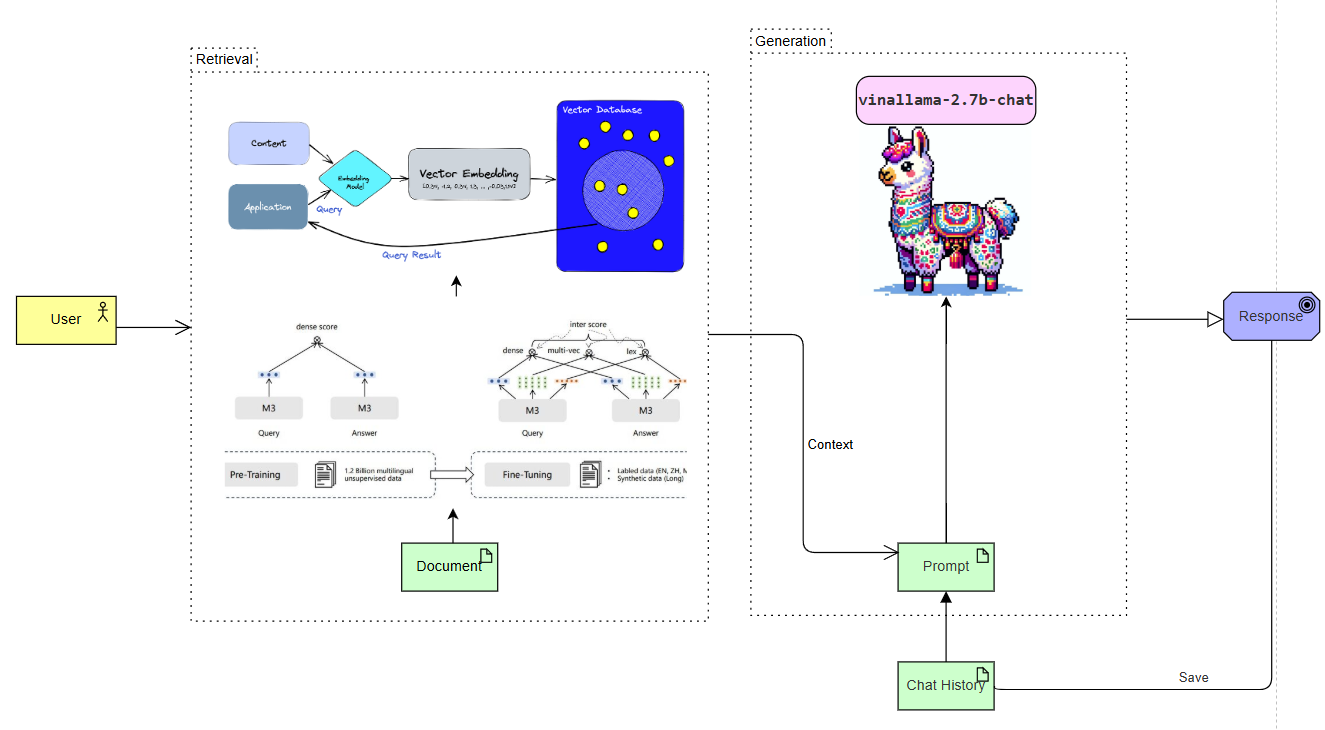
\includegraphics[width=0.95\linewidth]{bibliography/Figure/system-architech.png}
    \caption{System architecture of the proposed RAG-based consulting assistant using LangChain and vinallama-2.7b-chat.}
    \label{fig:architecture}
    \end{figure}
The overall architecture of our system is based on the Retrieval-Augmented Generation (RAG) framework, combining a retriever and a large language model (LLM) for more accurate and context-aware responses. The system consists of two main modules: Retrieval and Generation, as illustrated in Figure~\ref{fig:architecture}.

In the \textbf{Retrieval} module, when a user submits a query, the system encodes it into a vector embedding and compares it against a pre-built FAISS vector database. This database contains vectorized embeddings of documents that were preprocessed and selected from sources related to child development and mental health. The retrieval process employs a search method using \texttt{search\_type = "similarity"} to identify documents that exhibit a high degree of relevance to the input query. Only documents that meet a predefined similarity score threshold (\texttt{score\_threshold}) are selected. These documents are then compiled into a context that is passed to the Generation module for further processing.

The \textbf{Generation} module uses a Vietnamese LLM—\texttt{vinallama-2.7b-chat}—which has been fine-tuned on domain-specific instruction data to enhance its ability to generate context-aware and helpful responses in the field of child development and mental health. The retrieved documents, along with the current prompt, context from the retrieval module, and chat history, are passed to the model as input. The model then produces a response, which is returned to the user and optionally saved for continuous interaction.
    
\subsection{Component Implementation Details}
\label{sec:Component Implementation Details}
\subsubsection{Vector Database Construction}
\label{sec:Vector Database Construction}

This component is responsible for transforming raw documents into vector representations that can be efficiently queried using similarity search.


The process begins by loading and parsing a collection of PDF documents containing curated knowledge related to child development and mental health. Each document is then segmented into smaller chunks using a recursive text splitter with a chunk size of 1400 characters and an overlap of 200 characters. This overlapping strategy ensures that semantic context is preserved across boundaries and improves embedding consistency.

For vectorization, we employ the BGE-M3 model from the BAAI research group. It is a multilingual, fine-tuned model optimized for dense semantic retrieval. We utilize the SentenceTransformer interface to embed both the query and the document chunks.

All embeddings are normalized and stored in a FAISS vector database. This structure enables fast approximate nearest-neighbor (ANN) search. Prior to saving, the system verifies the integrity of the index by checking the alignment between document chunks and vector entries.

To further ensure data quality and minimize retrieval noise, we test the resulting vector store with a sample query. Any failure during the process triggers an automatic cleanup of the invalid store to prevent corrupted data from affecting future interactions.
\subsubsection{LLM Fine-Tuning}
\label{sec:LLM Fine-Tuning}

Pretrained base models such as VinaLLaMA, Vistral-7B, SeaLLMs, and Dama-2 were loaded from Hugging Face repositories. To reduce memory consumption and accelerate training, all models were quantized to 8-bit (int8) precision using bitsandbytes.

The training process applies Low-Rank Adaptation (LoRA) for parameter-efficient fine-tuning. Common attention and feedforward modules (e.g., \texttt{q\_proj}, \texttt{v\_proj}, \texttt{k\_proj}, \texttt{o\_proj}) were targeted for adaptation to maintain general language capabilities while enabling task-specific learning.

To ensure training data quality, the input dataset was filtered by computing cosine similarity between instruction and response pairs using a pretrained embedding model. Pairs with similarity scores below a specified \texttt{score\_threshold} (e.g., 0.9) were removed to eliminate noisy or inconsistent samples.

A 5-fold cross-validation strategy was employed to assess the robustness and generalization performance of each fine-tuned model. The dataset was split accordingly, and fine-tuning was performed independently on each fold.

Evaluation metrics used in this study include:

\vspace{1em}
\noindent \textbf{\textit{ROUGE-1}}\\

\textbf{Formula:}

\begin{equation}
\text{ROUGE-1} = \frac{\sum_{g \in G_1(R)} \min \left( \text{Count}_C(g), \text{Count}_R(g) \right)}{\sum_{g \in G_1(R)} \text{Count}_R(g)}
\end{equation}

\textbf{Explanation:}
\begin{itemize}
  \item $G_1(R)$ is the set of all \textit{unigrams} (single words) in the reference text $R$.
  \item $\text{Count}_C(g)$ is the number of times unigram $g$ appears in the candidate text $C$.
  \item $\text{Count}_R(g)$ is the number of times unigram $g$ appears in the reference text $R$.
  \item The numerator sums the number of overlapping unigrams between $C$ and $R$, using the minimum count from each to avoid overcounting.
  \item The denominator is the total number of unigrams in the reference, including duplicates.
\end{itemize}

\textbf{Interpretation:}

ROUGE-1 measures the unigram recall — how much of the reference content is covered by the candidate. The score ranges from $0$ to $1$:
\begin{itemize}
  \item ROUGE-1 = 1 means all reference words appear in the candidate.
  \item ROUGE-1 = 0 means there is no unigram overlap between candidate and reference.
\end{itemize}

\vspace{1em}
\noindent \textbf{\textit{ROUGE-2}}\\

\textbf{Formula:}

\begin{equation}
\text{ROUGE-2} = \frac{\sum_{g \in G_2(R)} \min \left( \text{Count}_C(g), \text{Count}_R(g) \right)}{\sum_{g \in G_2(R)} \text{Count}_R(g)}
\end{equation}

\textbf{Explanation:}
\begin{itemize}
  \item $G_2(R)$ is the set of all \textit{bigrams} (pairs of consecutive words) in the reference text $R$.
  \item $\text{Count}_C(g)$ is the number of times bigram $g$ appears in the candidate text $C$.
  \item $\text{Count}_R(g)$ is the number of times bigram $g$ appears in the reference text $R$.
  \item The numerator counts the number of overlapping bigrams between $C$ and $R$, taking the minimum count to avoid duplication.
  \item The denominator is the total number of bigrams in the reference (including repeated ones).
\end{itemize}

\textbf{Interpretation:}

ROUGE-2 measures the bigram-level recall — how many bigram phrases from the reference appear in the candidate. It focuses more on fluency and local word ordering compared to ROUGE-1. The score ranges from $0$ to $1$, where:
\begin{itemize}
  \item ROUGE-2 = 1 means every bigram in the reference also exists in the candidate.
  \item ROUGE-2 = 0 means there is no bigram overlap at all.
\end{itemize}
\vspace{1em}
\noindent \textbf{\textit{ROUGE-L}}\\

\textbf{Formula:}

\begin{align}
P_{\text{LCS}} &= \frac{\text{LCS}(C, R)}{|C|}, \quad
R_{\text{LCS}} = \frac{\text{LCS}(C, R)}{|R|} \\
\text{ROUGE-L} &= \frac{(1 + \beta^2) \cdot P_{\text{LCS}} \cdot R_{\text{LCS}}}{\beta^2 \cdot P_{\text{LCS}} + R_{\text{LCS}}}
\end{align}

\textbf{Explanation:}
\begin{itemize}
  \item $\text{LCS}(C, R)$ is the length of the \textit{Longest Common Subsequence} between the candidate text $C$ and the reference text $R$.
  \item $|C|$ and $|R|$ are the total number of words in the candidate and reference texts, respectively.
  \item $P_{\text{LCS}}$ is the LCS-based precision: the proportion of the candidate covered by the LCS.
  \item $R_{\text{LCS}}$ is the LCS-based recall: the proportion of the reference covered by the LCS.
  \item $\beta$ is a weighting factor to control the balance between recall and precision. Commonly, $\beta = 1$ to compute the F1-score.
\end{itemize}

\textbf{Interpretation:}

ROUGE-L captures the longest shared in-sequence word overlap between the candidate and the reference, regardless of contiguity. It is particularly useful for evaluating fluency and sequence alignment. A score of:
\begin{itemize}
  \item 1 indicates perfect in-order match between candidate and reference,
  \item 0 indicates no sequence overlap.
\end{itemize}
\vspace{1em}
\noindent \textbf{\textit{METEOR}}\\

\textbf{Formula:}

\begin{align}
P &= \frac{m}{|C|}, \quad R = \frac{m}{|R|} \\
F_{\text{mean}} &= \frac{10 \cdot P \cdot R}{R + 9 \cdot P} \\
\text{Penalty} &= \gamma \left( \frac{ch}{m} \right)^\beta \\
\text{METEOR} &= F_{\text{mean}} \cdot (1 - \text{Penalty})
\end{align}

\textbf{Explanation:}
\begin{itemize}
  \item $m$ is the number of matched unigrams between the candidate $C$ and reference $R$.
  \item $|C|$ and $|R|$ are the total number of unigrams in the candidate and reference texts, respectively.
  \item $P$ and $R$ are unigram-level precision and recall.
  \item $F_{\text{mean}}$ is a harmonic mean of $P$ and $R$, with recall weighted 9 times more than precision.
  \item $ch$ is the number of \textit{chunks} (i.e., contiguous matched subsequences in order).
  \item $\gamma$ and $\beta$ are hyperparameters that control how harshly disordered matches are penalized. Common values: $\gamma = 0.5$, $\beta = 3$.
  \item $\text{Penalty}$ increases as the number of chunks grows (i.e., when matches are more fragmented).
\end{itemize}

\textbf{Interpretation:}

METEOR measures both content matching and word order alignment. It rewards matches at the unigram level but penalizes disordered or fragmented alignments. A score of:
\begin{itemize}
  \item 1 indicates a perfect match in content and order,
  \item 0 indicates no match at all.
\end{itemize}
\vspace{1em}
\noindent \textbf{\textit{Cosine Similarity}}\\

\textbf{Formula:}

\begin{equation}
\text{CosineSim}(X, Y) = \frac{\sum_{i=1}^{n} X_i \cdot Y_i}{\sqrt{\sum_{i=1}^{n} X_i^2} \cdot \sqrt{\sum_{i=1}^{n} Y_i^2}}
\end{equation}

\textbf{Explanation:}
\begin{itemize}
  \item $X = (X_1, X_2, \dots, X_n)$ and $Y = (Y_1, Y_2, \dots, Y_n)$ are the vector representations of the candidate and reference texts, respectively.
  \item $X_i$ and $Y_i$ are the $i$-th components of vectors $X$ and $Y$ (e.g., embedding values).
  \item The numerator is the dot product between $X$ and $Y$.
  \item The denominator is the product of the Euclidean norms (magnitudes) of $X$ and $Y$.
\end{itemize}

\textbf{Interpretation:}

Cosine similarity measures the angle between two vectors in a high-dimensional space. It captures the semantic closeness between two texts regardless of their length. The score ranges from:
\begin{itemize}
  \item $1$: the vectors point in the same direction (perfect match),
  \item $0$: the vectors are orthogonal (no similarity),
  \item $-1$: the vectors are in opposite directions (rare in non-negative text embeddings).
\end{itemize}

\subsubsection{Integration with RAG and LangChain}

The final system was fully implemented by integrating the RAG (Retrieval-Augmented Generation) architecture with the LangChain framework, and deploying it as a production-ready chatbot using Ollama and FastAPI. Workflow of the system is shown in Figure~\ref{fig:architecture}.

\noindent\textbf{User Interaction via API Endpoint:}
The user submits a query to the API endpoint. This query is passed into the retrieval pipeline, which uses FAISS to identify the most semantically similar document chunks from the knowledge base, previously encoded using the BGE-M3 model.

\noindent\textbf{Retrieval Phase:}
The retriever searches using \texttt{search\_type = similarity} with $k$ and a \texttt{score\_threshold}. Only documents that satisfy the semantic similarity threshold are used to construct the context for the model.

\noindent\textbf{Prompt Construction:}
The prompt is constructed by concatenating the user query, the retrieved context, and the system message (including the conversation history).


\begin{tcolorbox}[title=Prompt Vietnamese Template Used in the System,fonttitle=\bfseries]
  \small
  \verb|<|im\_start|>|system
  
  Bạn là trợ lý AI chuyên về sức khỏe và tâm thần nhi khoa. Mục tiêu của bạn là cung cấp thông tin chính xác, dễ hiểu và hữu ích cho phụ huynh. Hãy tuân thủ các hướng dẫn sau:
  
  \begin{enumerate}
      \item \textbf{Ưu tiên Context:} Lấy thông tin từ phần \textbf{Context} được cung cấp làm nguồn chính để trả lời câu hỏi.
      \item \textbf{Bổ sung từ kiến thức của bạn:} Nếu Context không có thông tin, không đầy đủ, hoặc bạn cảm thấy kiến thức đã được huấn luyện (fine-tuned) của mình có thể làm rõ hơn hoặc bổ sung giá trị cho câu trả lời, hãy sử dụng nó. Thông tin bổ sung phải liên quan trực tiếp đến câu hỏi và lĩnh vực chuyên môn của bạn.
      \item \textbf{Chính xác và không bịa đặt:} Dù thông tin lấy từ Context hay từ kiến thức của bạn, nó phải chính xác và dựa trên cơ sở khoa học. Tuyệt đối không bịa đặt thông tin.
      \item \textbf{Tập trung vào câu hỏi:} Luôn trả lời trực tiếp vào câu hỏi \texttt{\{question\}}.
      \item \textbf{Khi không có thông tin:} Nếu cả Context và kiến thức đã huấn luyện của bạn đều không có thông tin để trả lời câu hỏi, hãy thông báo một cách lịch sự, ví dụ: ``Tôi rất tiếc, hiện tại tôi không có đủ thông tin về chủ đề này từ cả tài liệu được cung cấp lẫn kiến thức của mình.''
      \item \textbf{Diễn đạt:} Tự nhiên, không trích dẫn nguyên văn từ Context trừ khi đó là một định nghĩa quan trọng hoặc trích dẫn ngắn cần thiết.
      \item \textbf{Định dạng:} Rõ ràng, dùng gạch đầu dòng (-) hoặc số (1., 2.) nếu phù hợp, câu đầy đủ, đúng ngữ pháp.
      \item \textbf{Giọng điệu:} Ngôn ngữ đơn giản, thân thiện, cảm thông và hỗ trợ.
      \item \textbf{Lịch sử hội thoại:} Sử dụng lịch sử \texttt{\{chat\_history\}} để hiểu ngữ cảnh các câu hỏi trước đó, nhưng câu trả lời của bạn phải tập trung vào câu hỏi hiện tại.
      \item \textbf{Luôn kết thúc câu trả lời bằng:} ``Lưu ý: Thông tin từ AI chỉ mang tính tham khảo, không thay thế cho chẩn đoán hoặc tư vấn y tế từ bác sĩ chuyên khoa. Phụ huynh nên đưa trẻ đến gặp bác sĩ nhi khoa để được kiểm tra và tư vấn cụ thể.''
  \end{enumerate}
  
  \vspace{0.5em}
  \noindent\textbf{Context:} \texttt{\{context\}}\\
  \textbf{Chat History:} \texttt{\{chat\_history\}}
  
  \verb|<|im\_end|>|
  \verb|<|im\_start|>|user\\
  \texttt{\{question\}}\\
  \verb|<|im\_end|>|
  \verb|<|im\_start|>|assistant
\end{tcolorbox}
\subsection{Dataset}
  
\section{Results and Discussion}


\begin{thebibliography}{9}
    \bibitem{b1} Kailai Yang, Tianlin Zhang, Ziyan Kuang, Qianqian Xie, Jimin Huang, Sophia Ananiadou, "MentaLLaMA: Interpretable Mental Health Analysis on Social Media with Large Language Models," arXiv preprint arXiv:2309.13567v3, 2024
    \bibitem{b2} Albert Q. Jiang, Alexandre Sablayrolles, Arthur Mensch, Chris Bamford, Devendra Singh Chaplot, Diego de las Casas, Florian Bressand, Gianna Lengyel, Guillaume Lample, Lucile Saulnier, Lélio Renard Lavaud, Marie-Anne Lachaux, Pierre Stock, Teven Le Scao, Thibaut Lavril, Thomas Wang, Timothée Lacroix, William El Sayed, "Mistral 7B: Towards Efficient and High-Performance Language Models," arXiv preprint arXiv:2302.13971, 2023.
    \bibitem{b3} Quan Nguyen, Huy Pham, Dung Dao, "VinaLLaMA: LLaMA-based Vietnamese Foundation Model," arXiv preprint arXiv:2312.11011v1, 2023.
    \bibitem{b4} Xuan-Phi Nguyen, Wenxuan Zhang, Xin Li, Mahani Aljunied, Zhiqiang Hu, Chenhui Shen, Yew Ken Chia, Xingxuan Li, Jianyu Wang, Qingyu Tan, Liying Cheng, Guanzheng Chen, Yue Deng, Sen Yang, Chaoqun Liu, Hang Zhang, Lidong Bing, "SeaLLMs: Large Language Models for Southeast Asia," arXiv preprint arXiv:2312.16934v2, 2023.
    \bibitem{b5} Yunfan Gao, Yun Xiong, Xinyu Gao, Kangxiang Jia, Jinliu Pan, Yuxi Bi, Yi Dai, Jiawei Sun, Meng Wang, Haofen Wang, "Retrieval-Augmented Generation for Large Language Models: A Survey," arXiv preprint arXiv:2312.10997v5, 2024.
    \bibitem{b6} Liam Hebert, Lukasz Golab, Pascal Poupart, Robin Cohen, ``FedFormer: Contextual Federation with Attention in Reinforcement Learning''.
    \bibitem{b7} Jianlv Chen, Shitao Xiao, Peitian Zhang, Kun Luo, Defu Lian, Zheng Liu, "M3-Embedding: Multi-Linguality, Multi-Functionality, Multi-Granularity Text Embeddings Through Self-Knowledge Distillation," arXiv preprint arXiv:2402.03216v4, 2024.
    \bibitem{b8} Róbert Lakatos, Péter Pollner, András Hajdu, Tamás Joó, "Investigating the Performance of Retrieval-Augmented Generation and Fine-Tuning for the Development of AI-Driven Knowledge-Based Systems," arXiv preprint arXiv:2403.09727v1, 2024.
    \bibitem{b9} Harald Steck, Chaitanya Ekanadham, Nathan Kallus, "Is Cosine-Similarity of Embeddings Really About Similarity?" arXiv preprint arXiv:2403.05440v1, 2024.
    \bibitem{b10} Li, H., Li, X., Hu, P., Lei, Y., Li, C., Zhou, Y., … \& Zhou, Y. (2023). ``Boosting Multi-modal Model Performance with Adaptive Gradient Modulation''. arXiv preprint arXiv:2308.07686.
\end{thebibliography}

\end{document}
